\documentclass{beamer}

\usepackage[export]{adjustbox}
\usepackage{amsmath,amsthm,amssymb,amsfonts}
\usepackage[backend=biber, style=apa]{biblatex}
\usepackage{caption}
\usepackage[T1]{fontenc}
\usepackage{graphicx}
\usepackage{lmodern}
\usepackage[outputdir=dist]{minted}
\usepackage{ru}
\usepackage{url}
\usepackage{xpatch,letltxmacro}
\usepackage{stmaryrd}
\usepackage{wrapfig}

\newcommand{\cd}[1]{\texttt{#1}}

\setminted{fontsize=\small}
\LetLtxMacro{\cminted}{\minted}
\let\endcminted\endminted
\xpretocmd{\cminted}{\RecustomVerbatimEnvironment{Verbatim}{BVerbatim}{}}{}{}

\mode<presentation>{}

\title{\textbf{Compiler Construction: Lexical analyses}}

\author{Quinten Cabo, Marijn van Wezel}

\institute{Radboud University Nijmegen}
\date{27 February 2024}

\begin{document}

\setbeamercovered{transparent}
\setbeamercolor{alerted text}{fg=black}
\setbeamerfont{alerted text}{series=\bfseries}

\frame{\titlepage}

\begin{frame}
  \frametitle{What was a compiler again?}
  
  \begin{center}
  \only<1>{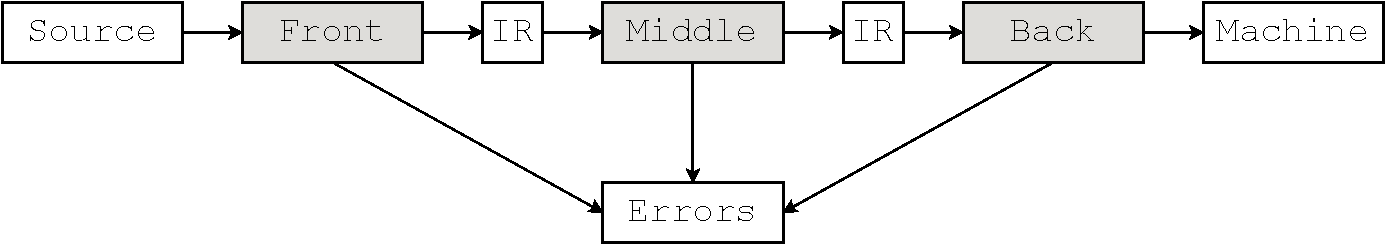
\includegraphics[width=300px]{figures/compiler_phases.pdf}}
  \only<2>{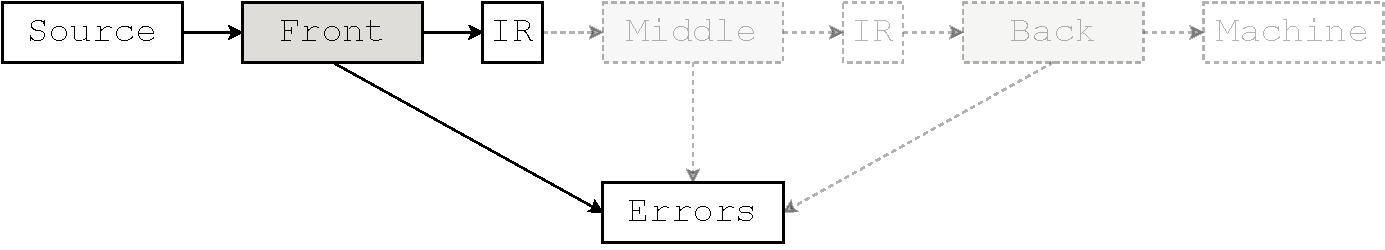
\includegraphics[width=300px]{figures/compiler_phases_highlighted.pdf}}
  \end{center}
\end{frame}

\begin{frame}<1>[label=the-goal]
  \frametitle{The goal}

  \begin{itemize}[<+->]
    \item \alert<1>{Given some arbitrary string of characters,}
    \item \alert<2>{analyse this string,}
    \item \alert<3>{produce an abstract syntax tree,}
    \item \alert<4>{or give an error.}
  \end{itemize}
\end{frame}

\begin{frame}[fragile]
  \frametitle{String of characters: Examples}

  \begin{onlyenv}<1>
    \begin{minted}{text}
      sum(l:[Int]): Int {
        if (isEmpty(l.tl)) {
          return l.hd;
        }

        return l.hd + sum(l.tl);
      }
    \end{minted}
  \end{onlyenv}

  \begin{onlyenv}<2>
    \begin{minted}{text}
      product(list:[Int]): Int {
        if (isEmpty(list)) {
          return 1;
        }

        return list.hd * product(list.tl);
      }
    \end{minted}
  \end{onlyenv}

  \begin{onlyenv}<3>
    \begin{minted}{text}
      product(list:[Int]: Int {
        if (isEmpty(list)) {
          return 1;
        }

        return list.hd * product(list.tl);
      }
    \end{minted}
  \end{onlyenv}
\end{frame}

\againframe<2>{the-goal}

\begin{frame}
  \frametitle{Analysis: Haskell}

  We chose \textit{Haskell} to implement our parser (and the rest of our compiler):

  \begin{itemize}[<+->]
    \item Algebraic data types;
    \item High level of abstraction;
    \item Good tooling and library support;
    \item \textbf{Functional parser combinators}.
  \end{itemize}
\end{frame}

\begin{frame}
  \frametitle{Analysis: Functional parser combinators}

  Parser combinators work through \textit{function composition}.

  \begin{center}
    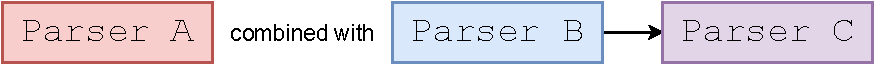
\includegraphics[width=300px]{figures/parser_combinator.pdf}
  \end{center}
\end{frame}

\begin{frame}
  \frametitle{Analysis: Megaparsec}

  \begin{figure}
    \begin{center}
      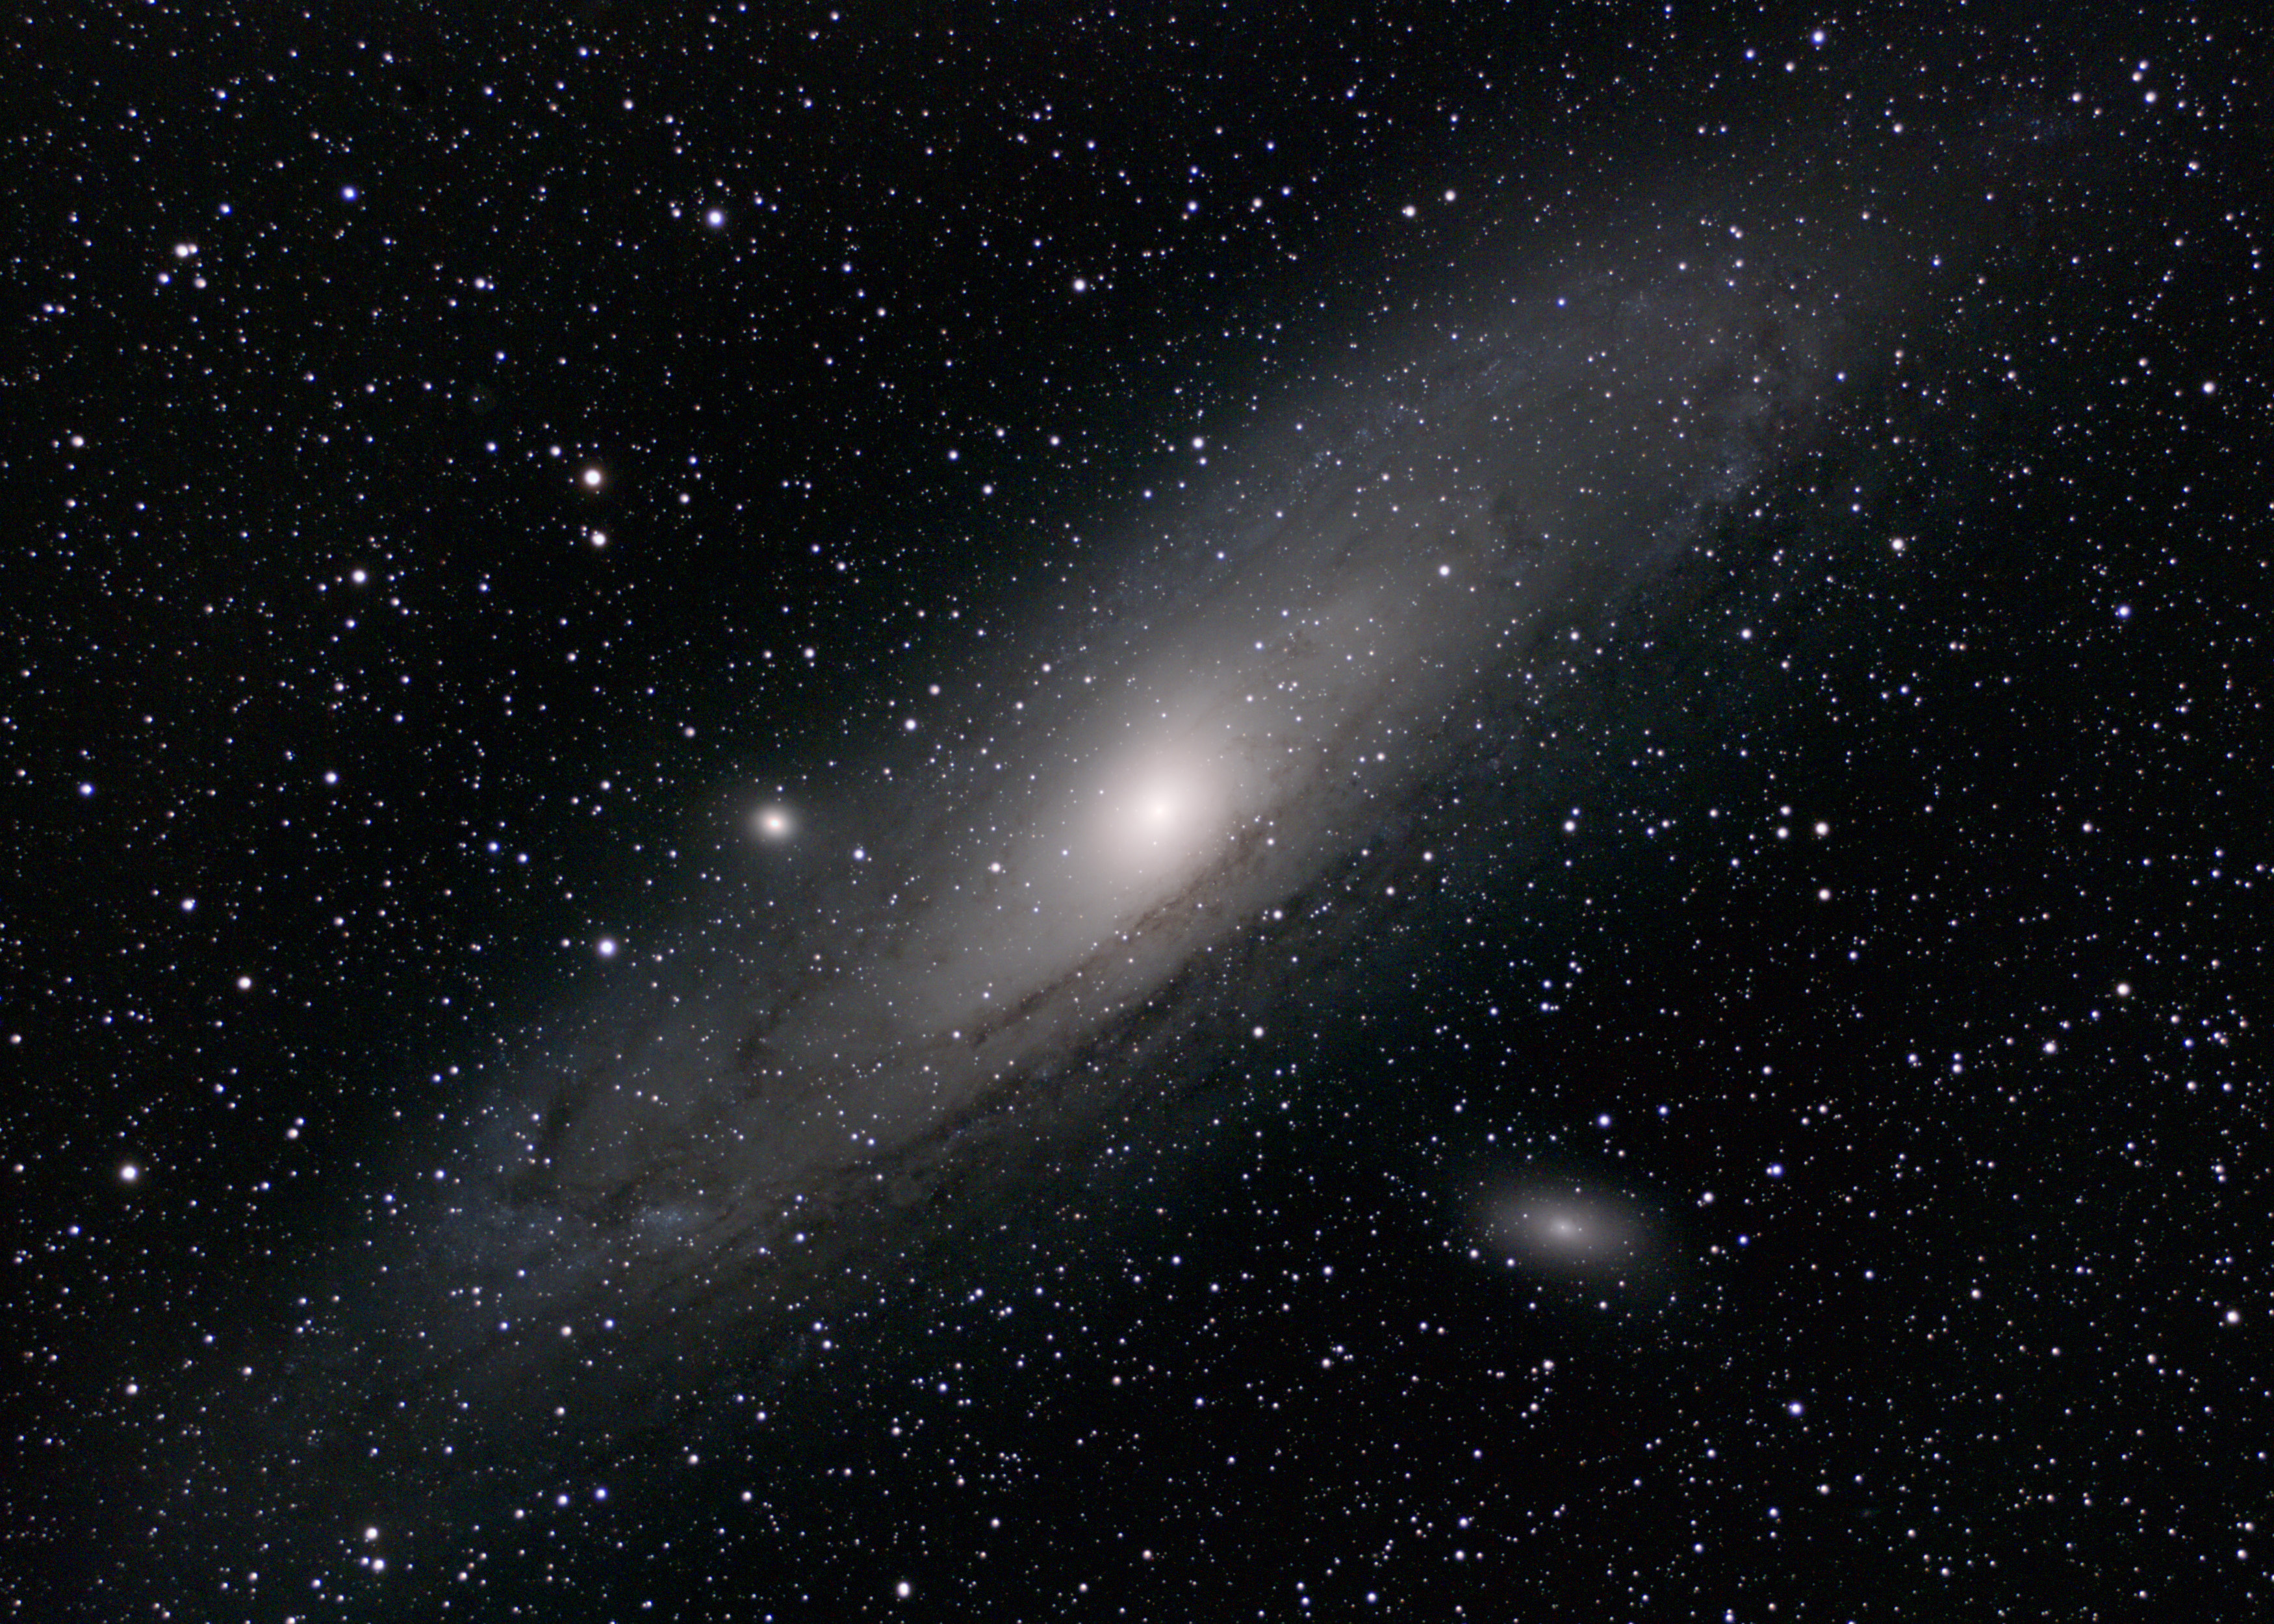
\includegraphics[width=0.7\textwidth]{figures/andromeda.jpg}
      \captionsetup{labelformat=empty}
      \caption{The Andromeda Galaxy is roughly one \textbf{megaparsec} away (Torben Hansen, CC-BY-2.0).}
    \end{center}
  \end{figure}
\end{frame}

\begin{frame}
  \frametitle{Analysis: Megaparsec}

  \begin{itemize}[<+->]
    \item Informal successor of Parsec;
    \item Does much of the heavy lifting;
    \item Large collection of combinators;
    \item Decent error messages out-of-the-box;
    \item \mintinline{text}{makeExprParser} 
  \end{itemize}
\end{frame}

\begin{frame}
  \frametitle{Analysis: Tokenless parsing}

  % whitespace
  % symbols
  % examples
  % megaparsec only removes whitespace at end
\end{frame}

\begin{frame}
  \frametitle{Analysis: Generating expression parsers}

  % field as expression
\end{frame}

\begin{frame}[fragile]
  \frametitle{Analysis: Testing the parser}

  hspec example:

    \begin{minted}{text}
describe "pTrue" $ do
  it "parses the string 'true' as TrueLit" $ do
      parse pTrue "test.spl" "false" `shouldParse` TrueLit

  it "doesn't parse anything else" $ do
      parse pTrue "test.spl" `shouldFailOn` "false"
      parse pTrue "test.spl" `shouldFailOn` "fa"
      parse pTrue "test.spl" `shouldFailOn` "tru"

    \end{minted}
\end{frame}

\begin{frame}[fragile]
  \frametitle{Analysis: Testing the parser output}

  % hspec example Make an error on purpose with true and false.

    \begin{minted}{text}

pTrue
  parses the string 'true' as TrueLit [x]

Failures:

  app/Test/Parser/Expr.hs:132:48: 
  1) Parser.Parser.Parser.Expr.pTrue parses 
     the string 'true' as TrueLit
       expected: TrueLit
       but parsing failed with error:
         test.spl:1:1:
           |
         1 | false
           | ^^^^
         unexpected "fals"
         expecting "true"
    \end{minted}
\end{frame}

\begin{frame}[fragile]
  \frametitle{Analysis: Testing the parser}

  % hspec example

    \begin{minted}{text}
describe "pTrue" $ do
  it "parses the string 'true' as TrueLit" $ do
      parse pTrue "test.spl" "true" `shouldParse` TrueLit
    \end{minted}
\end{frame}

\begin{frame}[fragile]
  \frametitle{Analysis: Testing the parser}

  % hspec example

    \begin{minted}{text}
  pTrue
    parses the string 'true' as TrueLit [v]
    doesn't parse anything else [v]
  pFalse
    parses the string 'true' as TrueLit [v]
    doesn't parse anything else [v]
  pInt
    parses an integer [v]
    parses a signed integer [v]
    discards trailing whitespace [v]

Finished in 0.0091 seconds
88 examples, 0 failures
    \end{minted}
\end{frame}



\againframe<3>{the-goal}

\begin{frame}[fragile]
  \frametitle{Abstract syntax tree}
  % started with AST early by looking at examples of SPL source
  \begin{onlyenv}<1>
    \begin{minted}{text}
type Program = undefined
data Type = undefined
data Decl = undefined
data Stmt = undefined
data Expr = undefined
data UnaryOp = undefined
data BinOp = undefined
data Variable = undefined
data Literal = undefined
% Field
    \end{minted}
  \end{onlyenv}

  % started with literals
\begin{onlyenv}<2>
 \begin{minted}{text} 
data Literal =
      TrueLit               -- true
    | FalseLit              -- false
    | IntLit Int            -- 10, -10, +10
    | FloatLit Float        -- 10.0, -10.0, +10.0
    | CharLit Char          -- 'a'
    | TupleLit (Expr, Expr) -- (a, b)
    | EmptyListLit          -- []
    deriving (Eq, Show)
 \end{minted}
\end{onlyenv}

\begin{onlyenv}<3>
 \begin{minted}{text}
data Expr =
      BinOp BinOp Expr Expr      -- a + b
    | UnaryOp UnaryOp Expr       -- + a
    | AssignExpr Variable Expr   -- a = b
    | FunctionCall String [Expr] -- f()
    | VariableExpr Variable      -- a, a.tl, a.hd
    | LiteralExpr Literal        -- 10
    deriving (Eq, Show) 
  \end{minted}
\end{onlyenv}

% We then needed to define operations and variables

\begin{onlyenv}<4>

 \begin{columns}
  \column{0.5\textwidth}
    \begin{minted}{text}
data UnaryOp = 
    Negate            -- !a
  | FieldAccess Field -- .hd, .tl
  deriving (Eq, Show)
    \end{minted}

\column{0.5\textwidth}
  \begin{minted}{text}
data BinOp =
      Mul   -- '*'
    | Div   -- '/'
    | Mod   -- '\%'
    | Add   -- '+'
    | Sub   -- '-' 
    | Cons  -- ':'
    | Gt    -- '>'
    | Gte   -- '>='
    | Lt    -- '<'
    | Lte   -- '<='
    | Eq    -- '=='
    | Neq   -- '!='
    | And   -- '\&\&'
    | Or    -- '||'
    deriving (Eq, Show)
  \end{minted}
\end{columns}
\end{onlyenv}

\begin{onlyenv}<5>
  \begin{minted}{text}
data Variable = 
      Identifier String (Maybe Field) -- a, a.hd, a.tl
    deriving (Eq, Show)

data Field =
      HeadField -- hd
    | TailField -- tl
    deriving (Eq, Show)
  \end{minted}
\end{onlyenv}

\begin{onlyenv}<6>
  \begin{minted}{text}
data Stmt =
  ReturnStmt (Maybe Expr)           -- return a;
| IfStmt Expr [Stmt] (Maybe [Stmt]) -- if (a) {b} else {c}
| WhileStmt Expr [Stmt]             -- while (a) {b}
| ExprStmt Expr                     -- a;
| VarStmt (Maybe Type) String Expr  -- var hello = 'h':'i':[]
deriving (Eq, Show)
  \end{minted}
\end{onlyenv}

\begin{onlyenv}<7>

  % Add types
\begin{columns}
  \column{0.5\textwidth}
  \begin{minted}{text}
data Stmt =
  ReturnStmt (Maybe Expr)           
| IfStmt Expr [Stmt] (Maybe [Stmt]) 
| WhileStmt Expr [Stmt]            
| ExprStmt Expr                   
| VarStmt (Maybe Type) String Expr
deriving (Eq, Show)
\end{minted}

\column{0.5\textwidth}
  \begin{minted}{text}
  data Type =
    IntType          -- Int
  | CharType         -- Char
    | BoolType         -- Bool
  | VoidType         -- Void
  | TupleType Type Type-- (a, b)
  | ListType Type       -- [a]
  | TypeVar String      -- a
  deriving (Eq, Show)
  \end{minted}
\end{columns}
\end{onlyenv}

\begin{onlyenv}<8,9>
  \begin{minted}{text}
    -- a(b : c, d : e) : Bool {
    --     f();
    -- }
    data Decl = 
      FunDecl String (Maybe Type) [(String, Maybe Type)] [Stmt]
      deriving (Eq, Show)
  \end{minted}
\end{onlyenv}
\begin{onlyenv}<9>
  \begin{minted}{text} 



    type Program = [Decl] 
  \end{minted}
\end{onlyenv}



\end{frame}

\begin{frame}[fragile]
  \frametitle{Abstract syntax tree - example}
  \begin{onlyenv}<1>
  \begin{minted}{text}
    fib(n : Int) : Int {
      if (n == 0) {
          return 0;
      }
      if (n == 1) {
          if (true) {
              print('h':'i':[]);
          }
          return 1;
      }
      return fib(n - 1) + fib(n - 2);
    }
  \end{minted}
  \end{onlyenv}

  \begin{onlyenv}<2>
  \begin{minted}{text}
    [FunDecl "fib" (Just IntType) [("n",Just IntType)] 
     [IfStmt (BinOp Eq (VariableExpr (Identifier "n" Nothing)) 
             (LiteralExpr (IntLit 0))) 
             [ReturnStmt (Just (LiteralExpr (IntLit 0)))] Nothing,
      IfStmt (BinOp Eq (VariableExpr (Identifier "n" Nothing))
             (LiteralExpr (IntLit 1))) 
             [IfStmt (LiteralExpr TrueLit) [
                ExprStmt (FunctionCall "print" [BinOp Cons (LiteralExpr (CharLit 'h'))
                 (BinOp Cons (LiteralExpr (CharLit 'i'))
                  (LiteralExpr EmptyListLit))])] Nothing,
              ReturnStmt (Just (LiteralExpr (IntLit 1)))] Nothing,
               ReturnStmt (Just (BinOp Add (FunctionCall "fib"
                    [BinOp Sub (VariableExpr (Identifier "n" Nothing))
                    (LiteralExpr (IntLit 1))]) 
                    (FunctionCall "fib" [BinOp Sub 
                    (VariableExpr (Identifier "n" Nothing)) 
                    (LiteralExpr (IntLit 2))])))]]
  \end{minted}
\end{onlyenv}

\end{frame}

\againframe<4>{the-goal}

\begin{frame}
  \frametitle{Error reporting}
\end{frame}

\begin{frame}[fragile]
  \frametitle{Pretty printer}

  \begin{onlyenv}<1,2>
  \begin{minted}{text}
    fib(n : Int) : Int {
      if (n == 0) {return 0;}


if    (n == 1) {
   if           (true)           {print('h':'i':[]);}
return 1;}return (fib(n - 1) + fib(n - 2));  }
    \end{minted}
  \end{onlyenv}

\begin{onlyenv}<3>
  \begin{minted}{text}
  fib(n : Int) : Int {
    if (n == 0) {
        return 0;
    }
    if (n == 1) {
        if (true) {
            print('h':'i':[]);
        }
        return 1;
    }
    return fib(n - 1) + fib(n - 2);

  }
    \end{minted}
  \end{onlyenv}
  \only<2>{
\includegraphics[width=55px]{figures/barf.png}}
  \only<3>{
\includegraphics[width=55px]{figures/happy.png}}
\end{frame}

\begin{frame}[fragile]
  % comments are hard
  \frametitle{Pretty printer - Comments}
    \begin{onlyenv}<1>
  \begin{minted}{text}
    fib(n : Int) : Int {
      if (n == 0) {return 0;}
    
/*    /| ________________
O|===|* >________________>
      \|                         */

if    (n == 1) { //                                  h   i 
   if /* always true? */  (true) /* hi */    {print('h':'i':[]);}
return 1;}return (fib(n - 1) + fib(n - 2));  }
    \end{minted}
  \end{onlyenv}
\begin{onlyenv}<2>
  \begin{minted}{text}
  fib(n : Int) : Int {
    if (n == 0) {
        return 0;
    }
    if (n == 1) {
        if (true) {
            print('h':'i':[]);
        }
        return 1;
    }
    return fib(n - 1) + fib(n - 2);

  }
    \end{minted}
  \end{onlyenv}
  \only<2>{
\includegraphics[width=55px]{figures/kinda_sad.png}}

  \begin{onlyenv}<3>
  \begin{minted}{text}
    type Program = ([Decl], [Comment])
                        -- start  end 
    data Comment = Single Int Int Int Int String
                 | Multi  Int Int Int Int String
    % Make the symbol parser fix it
  \end{minted}
  \end{onlyenv}

\end{frame}


\begin{frame}
  \begin{center}Questions?\end{center}
\end{frame}

\end{document}

